\documentclass[12pt,letterpaper]{article}

\usepackage[bookmarks=true]{hyperref}
\usepackage{graphicx}
\usepackage{geometry}
\usepackage{fontspec}
\usepackage{xunicode}
\usepackage{xltxtra}
\usepackage{color,colortbl}
\usepackage{url}
\usepackage[table]{xcolor}
\usepackage{multirow}
\usepackage{xtab}
\usepackage[final]{pdfpages}
\usepackage{subfigure}
\usepackage{amsmath,amssymb}


\definecolor{Gray}{gray}{0.9}

\defaultfontfeatures{Mapping=tex-text} % converts LaTeX specials (``quotes'' --- dashes etc.) to unicode

\setromanfont [Ligatures={Common}]{Cardo}
\setmonofont{Inconsolata}

% Set your name here
\def\name{Patrick J. Martin}

% Replace this with a link to your CV if you like, or set it empty
% (as in \def\footerlink{}) to remove the link in the footer:
\def\footerlink{}

% The following metadata will show up in the PDF properties
\definecolor{darkblue}{rgb}{0.0,0.0,0.5}
\hypersetup{
  colorlinks = true,
  linkcolor=darkblue,
  urlcolor = darkblue,
  pdfauthor = {\name},
  pdftitle = {\name: PJM Application},
  pdfpagemode = UseNone
}

\geometry{
  body={6.5in, 8.5in},
  left=1.0in,
  top=1.0in,
  bottom=1.0in
}

\subfigcapmargin = .5cm

% Customize page headers
\pagestyle{myheadings}
\markright{\name}
\thispagestyle{empty}

% Custom section fonts
\usepackage{sectsty}
\sectionfont{\rmfamily\mdseries\Large}
\subsectionfont{\rmfamily\mdseries\large}

% Don't indent paragraphs.
\setlength\parindent{0em}

% Make lists without bullets
\renewenvironment{itemize}{
  \begin{list}{}{
    \setlength{\leftmargin}{1.5em}
  }
}{
  \end{list}
}

% courtesy D. Hovemeyer
\newenvironment{denseItemize}{%
\begin{list}{}{\setlength{\itemsep}{0.4em}\setlength{\leftmargin}{1.5em}\setlength{\parsep}{0in}}}{\end{list}}
%\setlength{\topsep}{.1mm}

\begin{document}

\pagestyle{myheadings}
\markright{\name---Project 1: Boston Housing Prices}
\thispagestyle{empty}

%{\LARGE \name} \\
%\smallskip
%\smallskip
{\Large Project 1: Boston Housing Prices} \\ 
Patrick Martin \\
\rule{\columnwidth}{1pt}

\vspace{1em}

This project required synthesis of introductory modeling and evaluation material.
Using the provided code skeleton, I modified four sections of the code to collect basic statistics from provided data, implement a performance metric, analyze the learning curves and model complexity, and tune a \texttt{DecisionTreeRegressor} algorithm.

\section*{Statistical Analysis of Housing Data}

The Boston housing data contained {\bf 506} entries that each have {\bf 13} features. Using \texttt{numpy} array functions, I determined the following statistical measures:
\begin{itemize}
	\item Minimum home price = {\bf 5.0}
	\item Maximum home price = {\bf 50.0}
	\item Mean home price = {\bf 22.5328}
	\item Median home price = {\bf 21.2}
	\item Standard deviation = {\bf 9.188}
\end{itemize}

\section*{Model Evaluation}

Home prices are based on continuous numerical values (or, drawn from $\mathbb{R}$).
Consequently, predicting a new home price based on current home price data is a {\bf regression} problem.
Choosing an error-based metric fits the problem, since we want the prediction algorithm to place values as close as possible to comparable homes.
In particular, I selected the {\bf mean-squared error} metric to penalize incorrect predictions far more than an absolute error.
The other scoring mechanisms discussed in class (e.g. precision, recall) make most sense for classification problems, not regression. \\

When tuning the \texttt{DecisionTreeRegressor}, we must split the data into appropriately sized training and testing data, which in this case was split 70/30.
Performing this split was enabled by a simple function call to \verb|train_test_split|.
We need to split the data into randomly chosen bins of training/test sets to get the best performance possible.
If you do not do the split correctly, it will result in a learning algorithm with poor learning performance (too little training data) or poor validation (too little test data).
In general, machine learning algorithms need cross validation to tune the algorithm using more sub sets of data from the given set.
For example, $K$-fold cross validation will run $K$ experiments with a randomly chosen set of data.
It will also be validated $K$ times. \\

The cross validation tool we used in this project was \verb|GridSeachCV| that accepts a candidate algorithm, the parameters of interest, and a scoring function.
By leveraging a known algorithm, the best \verb|max_depth| of the \verb|DecisionTreeRegressor| is computed with an exhaustive search.
My particular implementation uses the same \verb|mean_squared_error| performance metric and passes in the \verb|max_depth| parameter array.

\section*{Model Performance}



\begin{figure}[h!]
	\centering
	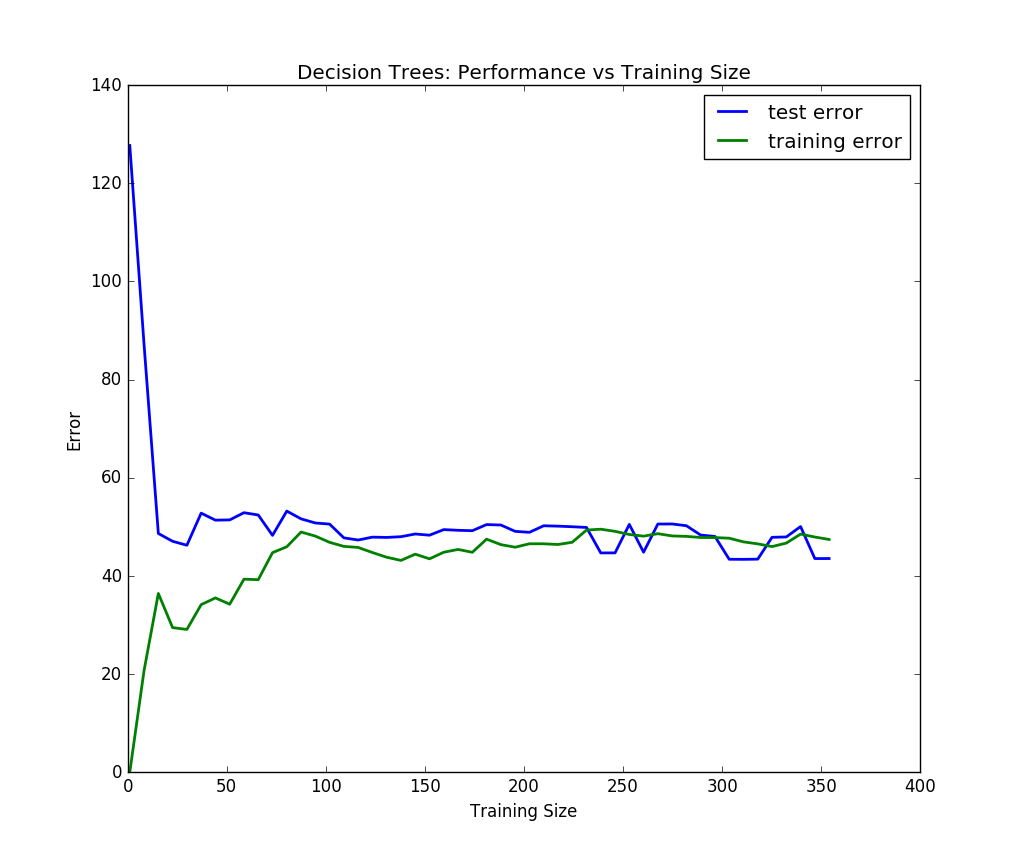
\includegraphics[width=0.6\textwidth]{dt-learningcurve-1.png}
	\caption{A plot of the training and test data error over size of training. This image is the initial run with the decision tree \texttt{depth = 1}.}
\end{figure}

\begin{figure}[h!]
	\centering
	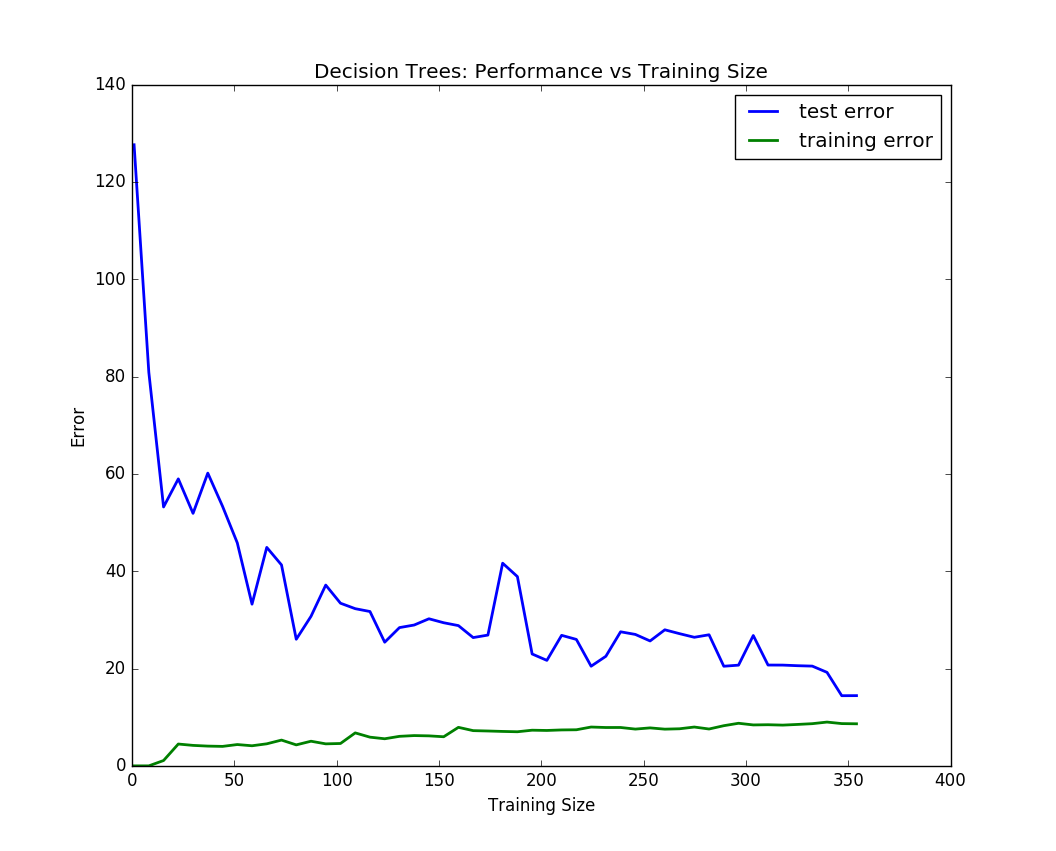
\includegraphics[width=0.6\textwidth]{dt-learningcurve-4.png}
	\caption{This image shows the error with a decision tree \texttt{depth = 4}.}
\end{figure}

\begin{figure}[h!]
	\centering
	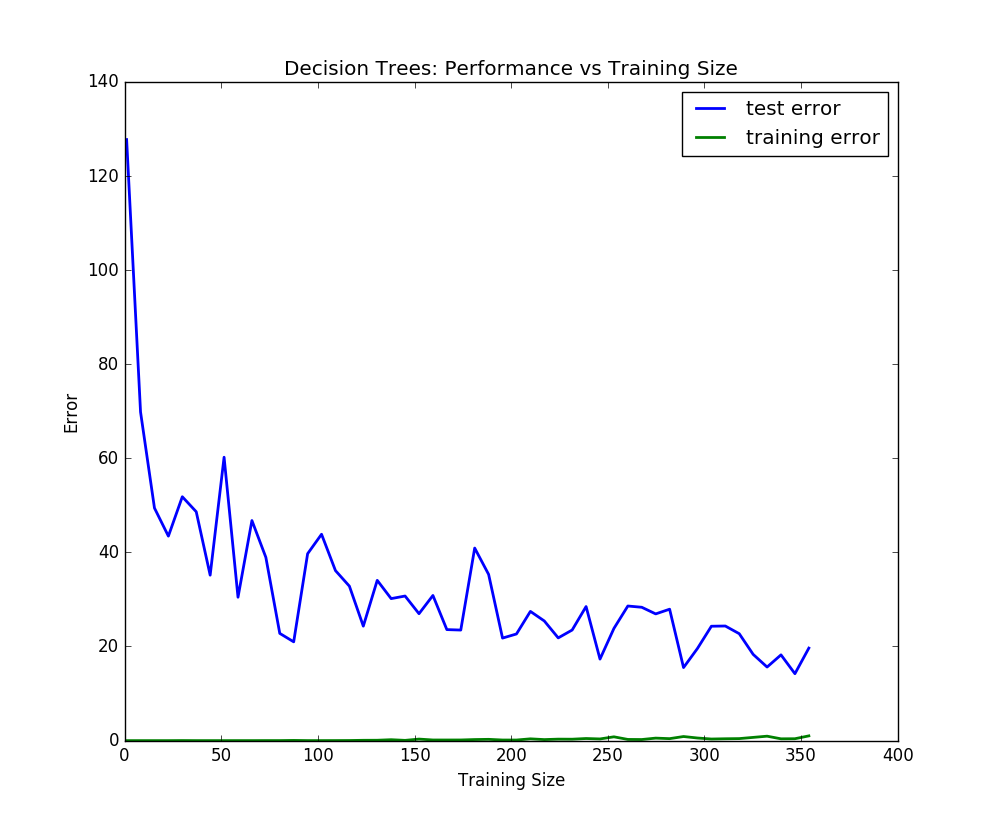
\includegraphics[width=0.6\textwidth]{dt-learningcurve-10.png}
	\caption{This image shows the error with a decision tree \texttt{depth = 10}.}
\end{figure}

\begin{figure}[h!]
	\centering
	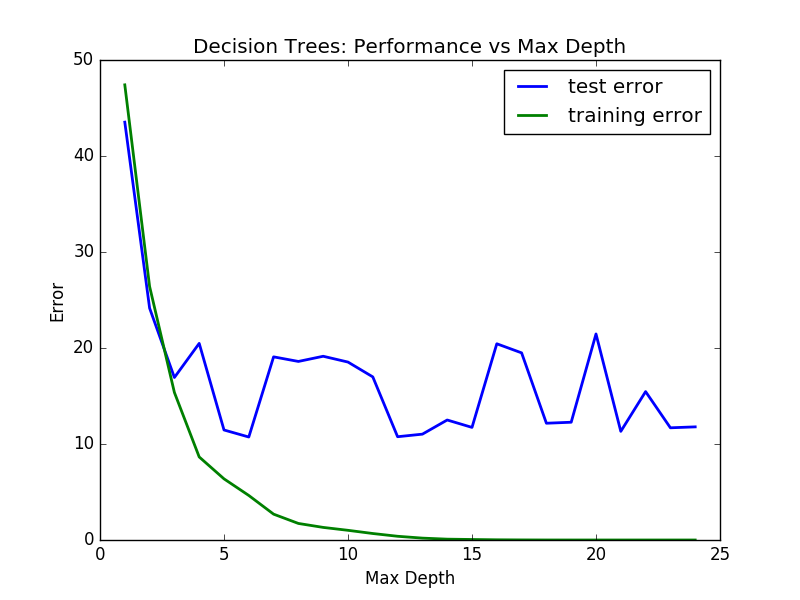
\includegraphics[width=0.6\textwidth]{model-complexity.png}
	\caption{A graph of the model complexity as the depth of the decision tree increases.}
\end{figure}


\end{document}